\capitulo{5}{Aspectos relevantes del desarrollo del proyecto}

%Este apartado pretende recoger los aspectos más interesantes del desarrollo del proyecto, comentados por los autores del mismo.
%Debe incluir desde la exposición del ciclo de vida utilizado, hasta los detalles de mayor relevancia de las fases de análisis, diseño e implementación.
%Se busca que no sea una mera operación de copiar y pegar diagramas y extractos del código fuente, sino que realmente se justifiquen los caminos de solución que se han tomado, especialmente aquellos que no sean triviales.
%Puede ser el lugar más adecuado para documentar los aspectos más interesantes del diseño y de la implementación, con un mayor hincapié en aspectos tales como el tipo de arquitectura elegido, los índices de las tablas de la base de datos, normalización y desnormalización, distribución en ficheros3, reglas de negocio dentro de las bases de datos (EDVHV GH GDWRV DFWLYDV), aspectos de desarrollo relacionados con el WWW...
%Este apartado, debe convertirse en el resumen de la experiencia práctica del proyecto, y por sí mismo justifica que la memoria se convierta en un documento útil, fuente de referencia para los autores, los tutores y futuros alumnos.

%Despliegue continuo - direccion de app en heroku. Sistema gratuito sirve para validar, pero no para explotar
%Diseño extensible
%Framework vaadin
%No responsive

%Comparacion de tfgs en la ubu, captura dde pantalla con comparativa tfg
Este capítulo recoge los aspectos más relevantes del ciclo de vida del proyecto y justifica los caminos que se han tomado durante el desarrollo. Se menciona el motivo de elección del proyecto, el modelo de ciclo de vida utilizado, una breve explicación de los aspectos de configuración del proyecto y el flujo de trabajo.

\section{Motivación de la elección y relación con asignaturas}

La elección de este trabajo fue motivada por su relación con la asignatura de \textit{Desarrollo Avanzado de Sistemas Software}. En esta se enseña como desarrollar software de calidad mediante el proceso de \textit{Administración de la calidad}, en la cual una de las actividades es el control de calidad. Este control se puede llevar a cabo mediante un proceso de medición. 

En este proyecto se han elegido métricas ya definidas para llevar un control sobre el ciclo de vida de uno o varios proyectos. Esto permite comprender el proceso de desarrollo, evaluarlo respecto a lo que se había planeado, predecir si los planes van por buen camino e identificar los defectos y mejorar la calidad del proceso. Además, esto ha podido ser comprobado, puesto que las mediciones realizadas por el software creado en este proyecto han servido para comparar este proceso con procesos de otros trabajos de fin de grado para saber si la evolución del proyecto era la adecuada.

Este proyecto tiene más relación con la asignatura de \textit{Desarrollo Avanzado de Sistemas Software}, pero también se han tomado referencias e ideas de las siguientes materias: 
\begin{itemize}
	\tightlist
	\item De \textit{Estadística}: el cálculo de cuartiles para calcular los valores umbrales de las métricas.
	\item De las asignaturas de \textit{Ingeniería del Software} y \textit{Análisis y Diseño de Sistemas}: todo lo relacionado con el ciclo de vida del software, el análisis de los requisitos y el modelado del sistema (diagramas de clases, diagramas de casos de uso, etc).
	\item De \textit{Interacción Hombre/Máquina}:  el diseño de la interfaz y las características que este debería alcanzar como usabilidad, la facilidad de aprendizaje, simplicidad, adaptabilidad, etc.
	\item De \textit{Gestión de Proyectos}: mayoritariamente el modelo de ciclo de vida del software: Scrum.
	\item De \textit{Diseño y Mantenimiento del Software}, el uso de patrones de diseño para mejorar la calidad de código y mantener los principios SOLID  \footnote{Single responsability, Open/Closed, Liskov substitution, Interface segregation, Dependency inversion} y de \textit{Desarrollo Avanzado de Sistemas Software} la naturaleza del trabajo, las revisiones automáticas de calidad de código por medio de métricas y la importancia de la refactorización al detectar defectos de diseño.
	\item \textit{Validación y Pruebas} en la construcción de la batería de pruebas.
	\item \textit{Sistemas Distribuidos} ha ayudado en el uso de Maven y en la construcción de una aplicación Web.
	\item \textit{Metodología de la Programación} y \textit{Estructuras de Datos} han contribuido en cuanto a la construcción de una aplicación en un lenguaje Orientado a Objetos.
\end{itemize}

\section{Modelo de ciclo de vida}

Tras la elección del proyecto se acordó definir una evolución que siga las bases del modelo \textit{\textbf{Scrum}}, tomando un proceso de desarrollo incremental con revisión de las iteraciones cada dos semanas (la duración del sprint). Estas revisiones se realizan por medio de reuniones que constaban de dos partes:
\begin{description}
	\item [Revisión del sprint:] Se revisa el incremento generado como resultado del sprint, se describen los problemas que hubo durante su desarrollo y se plantean mejoras sobre el incremento (se puede modificar la pila del producto o \textit{product backlog} \footnote{Lista de requisitos de usuario que, a partir de la visión inicial del producto, crece y evoluciona durante el desarrollo \citep{scrum_master_scrum_2019}}) y soluciones a estos problemas.
	\item [Planificación del siguiente sprint:] Se definen las tareas que se deben ejecutar durante el siguiente sprint. Estas tareas en \textit{Scrum} se recogen en la pila del sprint o \textit{sprint backlog}.
\end{description}

Según la naturaleza de los sprints, en el proceso del desarrollo se pueden diferenciar varias etapas:
\begin{itemize}
	\item  Una primera etapa de \textbf{investigación} de las herramientas que se utilizarán durante el proceso y de \textbf{configuración} del entorno de desarrollo.
	\item En la segunda etapa se aprecian tareas de \textbf{diseño e implementación} de la parte lógica de la aplicación. Se diseña el framework de conexión a forjas de repositorios, se implementa el framework descrito en \textit{Soporte de Métricas con Independencia del Lenguaje para la Inferencia de Refactorizaciones}  \citep{marticorena_sanchez_soporte_2005} para el cálculo de métricas y se diseñan los modelos de datos que serán utilizados por la aplicación.
	\item Durante la segunda etapa se apreció que se debía facilitar el \textbf{flujo de trabajo}, la comunicación entre tutor y alumno y facilitar las reuniones de revisión y planificación del sprint. Era preciso pausar la segunda etapa para dedicar un tiempo a estas tareas. Esto tuvo duración de un sprint y se realizaron tareas como:
		\begin{itemize}
			\item Configurar la gestión del proyecto con Maven \footnote{Gestor de proyectos software que ayuda en la construcción del proyecto, la generación de documentación, la generación de informes, la gestión de dependencias, la integración con un sistema de control de versiones, etc.}.
			\item Configurar los procesos de integración y despliegue continuo (CI/CD) con GitLab. En estos procesos se realizan actividades automáticamente cada cierto tiempo o cada vez que se realice algún cambio. Ejemplos de estas actividades serían: construir software (\textit{build}), realizar pruebas y revisar su cobertura, despliegue en caso de que se trate de una aplicación Web, revisar la calidad, etc.
			\item Realizar pruebas unitarias con JUnit y automatizar su ejecución gracias a Maven y los \textit{pipelines} \footnote{Definen las actividades de los procesos de CI/CD y las fases y el entorno en las que se ejecutarán} de GitLab.
			\item Configurar revisiones automáticas de calidad y de cobertura de las pruebas gracias a Maven, Codacy, JaCoCo y GitLab.
			\item Configurar un entorno en Heroku donde poder desplegar la aplicación entre las actividades de CI/CD y así poder ser revisada por el tutor fácilmente.
			\item Configurar badges \footnote{Distintivos que aportan información rápida sobre el estado del proyecto en ciertos aspectos como la cobertura, la calidad de código o el proceso de CI/CD y enlazan con la fuente de información} para representar el estado del proyecto en cuanto a calidad de código, cobertura, despliegue y los trabajos de CI/CD.
		\end{itemize}
	\item Etapa  de diseño e implementación de la \textbf{interfaz gráfica} y \textbf{mejora de funcionalidades}. A menudo, estas mejoras precisaban de modificaciones en la parte lógica de la aplicación.
	\item Etapa de \textbf{documentación} en la que se escribe la memoria y los anexos. También se preparan videotutoriales y manuales de usuario.
\end{itemize}

Para más detalles se puede consultar el \textit{Anexo A - Plan de Proyecto Software}. En este se muestra más información sobre estos sprints y el ciclo de vida del proyecto.

\section{Gestión del proyecto}

En esta sección se exponen y se justifican las principales decisiones que se han tomado en cuanto a la configuración del proyecto.

\subsection{Aplicación Web}

Para alcanzar los objetivos del proyecto se ha decidido implementar una aplicación Web. La principal diferencia es que no se instala en un equipo local sino que se accede a la aplicación desde un navegador Web, después de que esta haya sido desplegada en un servidor. Esto tiene varias ventajas: 
\begin{itemize}
	\tightlist
	\item El usuario no necesita instalar la aplicación y puede acceder a ella directamente desde el navegador, esto evita costes de tiempo y de recursos del computador.
	\item  Portabilidad. Es posible que una aplicación de escritorio no pueda ser instalada en ciertos computadores debido a los recursos de los que disponen, el sistema operativo u otros factores. Una aplicación Web solo depende del navegador que tenga instalado el computador y, normalmente, puede tener varios instalados. Además, se ha comprobado la portabilidad de navegador y la aplicación funciona en los principales navegadores: \textit{Mozilla Firefox}, \textit{Microsoft Edge}, \textit{Internet Explorer}, \textit{Google Chrome} y \textit{Opera}.
	\item Actualizaciones. Para actualizar una aplicación Web, el usuario final no tiene que instalar la actualización. Sino que habrá un periodo de mantenimiento de aplicación, normalmente muy corto y fuera de horario de uso, en el que ningún usuario podrá acceder a la aplicación. Después de este periodo, todos los usuarios dispondrán de la actualización.
\end{itemize}

\subsection{Java 11}

El proyecto se iba a desarrollar en Java desde el principio, era uno de los requisitos no funcionales iniciales. La elección de la versión fue uno de los temas que se discutieron al inicio del proyecto. Java 8 era la versión más conocida y la más estable, pero recientemente había surgido la versión 11 de Java. 

Se escogió la versión 11, por ser la más reciente \footnote{Actualmente, la versión Java SE 12.0.2 es la más reciente}. Esto supuso un estudio de las versiones que se debían utilizar de las herramientas que requieren de Java, como Tomcat \footnote{Para desplegar aplicaciones con Java 11 se requiere de la versión 9.0.x de Tomcat} y algunas otras configuraciones. Por ejemplo, se tuvo que configurar el fichero \ruta{pom.xml} del proyecto para que Maven compile en la versión 11 de Java:

\begin{minipage}{\linewidth}
{\tiny
\begin{lstlisting}[breaklines]
...
<properties>
	<project.build.sourceEncoding>UTF-8</project.build.sourceEncoding>
	<project.reporting.outputEncoding>UTF-8</project.reporting.outputEncoding>
	<java.version>11</java.version>
</properties>
...
<build>
...
	<plugins>
		<plugin>
			<groupId>org.apache.maven.plugins</groupId>
			<artifactId>maven-compiler-plugin</artifactId>
			<configuration>
				<source>${java.version}</source>
				<target>${java.version}</target>
			</configuration>
			<version>3.8.0</version>
		</plugin>
		<plugin>
			<groupId>org.apache.maven.plugins</groupId>
			<artifactId>maven-war-plugin</artifactId>
			<version>3.2.2</version>
		</plugin>
		...
	</plugins>
	...
</build>
...
\end{lstlisting}
}
\end{minipage}

Y en Eclipse IDE habría que añadir manualmente el JRE desde la ventana Window/Preferences, como se muestra en la Fig. \ref{fig:M5_Eclipse_Java11}.

\imagen{M5_Eclipse_Java11}{Añadir Java 11 a Eclipse}

Sin embargo, como se comentó en el anterior capítulo: \ref{sect:4_1_1_HerramientasDesarrollo} --- \textit{Técnicas y herramientas}, tampoco se trabajó demasiado con las nuevas funcionalidades que trae Java 11, ya que ha sido posible compilar el artefacto final con Java 1.8 y solo han sido necesarios dos pequeños cambios:
\begin{itemize}
	\item De la versión 11 se ha utilizado el método \textit{isBlank()} de la clase \textit{String} \footnote{\url{https://docs.oracle.com/en/java/javase/11/docs/api/java.base/java/lang/String.html}}. Se diferencia de \textit{isEmpty()} en que no comprueba la longitud de la cadena y devuelve \textit{true} si es 0. Sino que devuelve \textit{true} si la longitud es 0, o si no es 0 pero todos los caracteres de la cadena son espacios en blanco.
	\item De la clase \textit{java.util.Optional} \footnote{\url{https://docs.oracle.com/en/java/javase/11/docs/api/java.base/java/util/Optional.html}}, soportada desde la versión 1.8, se utiliza la función \textit{orElseThrow()}, que se soporta desde la versión 10, por tanto habría que buscar una alternativa para pasar a la versión 1.8. La versión 11 trae a esta clase la función \textit{isEmpty()}.
\end{itemize}

Para saber más sobre las novedades de Java 11 es recomendable leer `\textit{JDK 11 Release Notes}' \citep{oracle_jdk_nodate}. También hay un artículo que explica las principales diferencias entre Java 8 y Java 11 llamado `\textit{De Java 8 a Java 11, ¿aún no te has migrado?}' \citep{del_hoyo_java_2019}.

\subsubsection{Trabajo con streams de Java}

Desde Java 1.8 se puede trabajar con Streams. En este proyecto se ha dado gran uso de ellos debido a que facilitan enormemente el procesamiento de grandes colecciones de datos. Estos permiten \textbf{filtrar} datos de una colección mediante un predicado, \textbf{ordenar} los datos mediante un comparador, \textbf{mapear} o \textbf{reducir} los datos mediante alguna función y \textbf{almacenarlos} en algún tipo de colección mediante un colector. El mapeo asocia cada dato del stream con un nuevo elemento, por ejemplo, de cada número de una colección numérica obtenemos su potencia de dos. Y la reducción es obtener un único resultado a partir del conjunto de datos, por ejemplo, obtener el máximo o la suma de todos los datos de un conjunto numérico.

A continuación se muestra una fracción de código de la aplicación en la que se usan los streams:\\
\begin{minipage}{\linewidth}
{\tiny
\begin{lstlisting}[breaklines]
...
return gitLabApi.getIssuesApi().getIssuesStream(projectId, new IssueFilter().withState(IssueState.CLOSED))
  .filter(issue -> issue.getCreatedAt() != null && issue.getClosedAt() != null)
  .map(issue -> (int) ((issue.getClosedAt().getTime() - issue.getCreatedAt().getTime()) / (1000 * 60 * 60 * 24 )))
  .collect(Collectors.toList());
...
\end{lstlisting}
}
\end{minipage}

En el ejemplo se obtiene de GitLab API un stream con las issues cerradas de un proyecto. De este se filtran y se obtienen las que tengan fecha de creación y fecha de cierre (\textit{filter}), se calcula de cada issue la diferencia en días entre la fecha de creación y la fecha de cierre (\textit{map}), y se recogen los resultados en una lista (\textit{collect}).

\subsubsection{Interfaces funcionales y funciones lambda de Java}

Otros de los aspectos de Java que se han estudiado y utilizado en este proyecto son las interfaces funcionales y funciones lambda. En la sección anterior ya vemos el uso de dos funciones lambda en el código mostrado (argumentos de las funciones \textit{filter} y \textit{map}).

El paquete \textit{java.util.function} \footnote{\url{https://docs.oracle.com/javase/8/docs/api/java/util/function/package-summary.html}} es soportado por Java desde la versión 1.8. Este paquete permite almacenar funciones en variables. Las funciones lambda son funciones anónimas con sintaxis \\
\begin{minipage}{\linewidth}
{\tiny
\begin{lstlisting}
(parametros) -> {cuerpo funcion lambda}
\end{lstlisting}
}
\end{minipage}
que no están declaradas en una clase y pueden ser utilizadas en cualquier parte, pasarse como parámetro a una función y ser almacenadas en variables. Las interfaces funcionales \footnote{\url{https://docs.oracle.com/javase/8/docs/api/java/lang/FunctionalInterface.html}} son interfaces con un único método, que es abstracto, llamado método funcional. Este método permite restringir los tipos de los parámetros y de los valores de retorno de una función lambda.

Estas han sido utilizadas en numerosas ocasiones tanto para los streams (como se observa en el código anterior), como en elementos de la interfaz gráfica y otros elementos sensibles a eventos:\\
\begin{minipage}{\linewidth}
{\tiny
\begin{lstlisting}[breaklines]
...
closeConnectionButton.addClickListener(event ->  
{
  if(rds.getConnectionType() != EnumConnectionType.NOT_CONNECTED) {
	try {
	  rds.disconnect();
	} catch (RepositoryDataSourceException e) {
		...
	}
  }
  close();
  connectionFormDialog.open();
});
...
\end{lstlisting}
}
\end{minipage}

También han sido utilizadas para almacenar funciones en variables, definiendo una interfaz funcional para restringir los tipos parámetros y de los resultados de la función. Un aspecto importante es que las variables que almacenen funciones NO se pueden serializar, por eso la variable \textit{EVAL\_FUNC\_GREATER\_THAN\_Q1} del código siguiente se ha marcado como \textit{transient} dentro de una clase que implementa \textit{Serializable}.

\begin{minipage}{\linewidth}
{\tiny
\begin{lstlisting}[breaklines]
...
public interface Metric extends Serializable {
 @FunctionalInterface
 public interface EvaluationFunction {
   EvaluationResult evaluate(IValue value, IValue minValue, IValue maxValue);
 }

 ...
 
 EvaluationResult evaluate(IValue measuredValue);

 EvaluationFunction getEvaluationFunction();
}

...
public abstract class NumericValueMetricTemplate implements Metric {
  ...
  protected transient static final EvaluationFunction EVAL_FUNC_GREATER_THAN_Q1 = 
    (measuredValue, minValue, maxValue) -> 
     {
      try {
        Double value, min;
	    value = ...
	    min = ...
	    if (value > min) return EvaluationResult.GOOD;
	    else if (value.equals(min)) return EvaluationResult.WARNING;
	    else return EvaluationResult.BAD;
	  } catch (Exception e){
	    return EvaluationResult.BAD;
	  }
    };
  ...
}
...
\end{lstlisting}
}
\end{minipage}

En el ejemplo anterior se almacena la forma en la que las métricas podrían valorarse. En este caso la métrica será dada como buena si supera el umbral inferior. Cada métrica podrá usar esta función o implementar una función propia. Los requisitos definidos en la interfaz funcional son que esa función deberá tener tres argumentos del tipo \textit{IValue} y devolver un resultado del tipo \textit{EvaluationResult}.

\subsection{Maven}

Maven es una herramienta de gestión de proyectos software. Esta herramienta facilita, a partir de un único fichero con extensión \textit{XML} llamado \ruta{pom.xml} \footnote{Project Object Model}:
\begin{itemize}
	\tightlist
	\item La construcción y compilación del proyecto
	\item La generación de documentación
	\item La generación de informes, por ejemplo, informes de cobertura
	\item La gestión de las dependencias del proyecto
	\item La integración con un sistema de control de versiones como Git, y el trabajo con repositorios remotos como GitLab o GitHub e incluso en repositorios \textit{self-hosted} \footnote{Repositorios almacenados en servidores gestionados por la propia empresa o equipo que desarrolla el software}
	\item La generación y distribución de \textit{releases}
\end{itemize}
La herramienta es capaz de crear la estructura de directorios del proyecto, administrar las dependencias y descargar las librerías necesarias. También es posible utilizar arquetipos, que son patrones o plantillas que se aplican en la infraestructura del proyecto. Esto reduce en gran medida los tiempos de configurar e implementar el entorno de desarrollo para poder centrarse en el desarrollo del código de nuestro proyecto. Además, es compatible con la mayoría de IDEs \footnote{Integrated Development Environment - Entorno de desarrollo integrado}. Por ejemplo, en este proyecto se ha trabajado sobre Eclipse IDE, el cual tiene muy buena integración con Maven, como se puede observar en la Fig. \ref{fig:M5_Eclipse_Maven}.

\imagen{M5_Eclipse_Maven}{Integración de Maven con Eclipse}

El inconveniente de Maven es el coste de aprendizaje. Es complicado definir el fichero \ruta{pom.xml}, y cada herramienta (Tomcat, Heroku, Codacy, JUnit, Vaadin, etc) tiene sus propias instrucciones de cómo integrar la herramienta al proyecto con Maven. Hay que tener mucha experiencia para manejar Maven con fluidez pero, una vez entendido como funciona, uno se da cuenta del tiempo que gana utilizando esta herramienta.

\subsection{Sistema de control de versiones}

Durante el desarrollo del proyecto se ha utilizado Git como sistema de control de versiones y en GitLab se ha alojado el repositorio Git remoto del proyecto.

En un proyecto software es difícil que falte este sistema. Se encarga de almacenar el código en un repositorio y llevar un historial de cambios en todos los archivos del proyecto. Esto permite a un equipo de desarrollo trabajar simultáneamente sin miedo a sobrescribir el trabajo del compañero. También registra los cambios, el autor de los mismos, la fecha y permite justificar el cambio. Este sistema es esencial para llevar a cabo un control sobre la evolución del proyecto.

El entorno de desarrollo \textit{Eclipse IDE for Java EE Developers} tiene instalado un plugin para poder trabajar con Git. Lo más cómodo es abrir la perspectiva Git desde el menú Window/Perspective/Open Perspective, la perspectiva se muestra en la Fig. \ref{fig:M5_Eclipse_Git} y permite trabajar cómodamente con Git. Como se puede observar incluye un listado de repositorios a la izquierda; un comparador de cambios en el centro dónde se puede ver las diferencias entre lo que hay almacenado en el repositorio después del último commit y lo que hay en el espacio de trabajo (\textit{workspace}) e incluso se puede editar y deshacer los cambios realizados; en la parte inferior hay varias pestañas, una de ellas permite ver el historial de cambios de un fichero y otra que permite: ver los ficheros modificados sin proteger mediante commit, indexar los ficheros, agregar un título y descripción al commit, realizar el commit y enviarlo al repositorio remoto.

\imagen{M5_Eclipse_Git}{Perspectiva Git en Eclipse IDE for Java EE Developers}

Es posible configurar Maven para trabajar con Git. Sin embargo, se ha preferido la perspectiva Git de Eclipse por ser un entorno más visual que un intérprete de comandos.

\subsection{Logging}

Un logger sirve para redireccionar a uno o varios dispositivos información sobre el funcionamiento del programa. Normalmente, esa información consiste en trazas de error, y esos dispositivos podrán ser la consola, ficheros, o una base de datos. Esto mejora la comprensión del funcionamiento de la aplicación, la mantenibilidad del sistema y la detección y corrección de errores.

En el entorno de desarrollo conviene mejor visualizar estos mensajes por consola para monitorizar el programa y realizar pruebas, mientras que en el entorno de producción, lo habitual es almacenar esta información en un dispositivo persistente en ficheros o en una base de datos. Esto permite al equipo de desarrollo conocer la traza de funcionamiento del sistema en caso de error o comportamiento inesperado en tiempo de explotación.

La información que se registra en un log se estructura por niveles, por ejemplo, de mayor a menor detalle:
\begin{description}
	\item[DEBUG.] Sirve para depurar la aplicación en entorno de desarrollo. Este nivel suele estar desactivado en tiempo de explotación.
	\item[INFO.] Sirve para dar información del estado del sistema en tiempo de explotación. Por ejemplo, el número de usuarios conectados a una aplicación multiusuario. No indica error, pero se podría detectar que en ciertos estados de la aplicación, ocurren más errores (p. ej. al llegar a un determinado número de usuarios conectados, la aplicación falla).
	\item[WARN.] Se utiliza para alertar sobre situaciones anómalas de las que de desean dejar constancia, pero que no afectan al funcionamiento del sistema. 
	\item[ERROR.] Dejan constancia de los errores del programa que han ocurrido sin impedir que se siga ejecutando.
	\item[FATAL.] Dejan constancia de errores críticos del sistema que, generalmente, abortan la ejecución del programa.
\end{description}

En este proyecto se han utilizado dos herramientas para este proceso:
\begin{itemize}
	\item SLF4J (\textit{Simple Logging Facade for Java}). Es una capa intermedia entre el logger (\ruta{java.util.logging}, \ruta{logback}, \ruta{log4j}, etc) y la aplicación, lo que permite poder cambiar de logger fácilmente en tiempo de despliegue, sin necesidad de realizar grandes cambios en el código de la aplicación.
	
	\item Log4j. Logger. Permite configurar este proceso (dispositivos de información, niveles y formato de los mensajes, etc) por medio de un fichero \textit{log4j2} con extensión \textit{XML}, \textit{JSON}, \textit{YAML} o \textit{Properties}. En este proyecto se configuró mediante un fichero con extensión \ruta{.properties} ubicado en \ruta{src/main/resources}.
\end{itemize}

Para utilizar estas herramientas, se deben añadir las dependencias correspondientes (\ruta{slf4j-api}, \ruta{log4j-slf4j-impl}, \ruta{log4j-core}) en el fichero \ruta{pom.xml} del proyecto. También se configuró Log4J a través del fichero \ruta{log4j2.properties} en la carpeta de recursos \ruta{src/main/resources} para redirigir los mensajes a un fichero con ruta \textit{log/log4.log}, y a la consola (solo se activa en desarrollo).

Para crear registros en el log, cada clase cuenta con un atributo:\\
\begin{minipage}{\linewidth}
{\tiny
\begin{lstlisting}[breaklines]
private static final Logger LOGGER = LoggerFactory.getLogger(MetricsService.class);
\end{lstlisting}
}
\end{minipage}
y para registrar un error solo es necesario realizar una llamada al logger en la que se le proporciona el nivel de error:\\
\begin{minipage}{\linewidth}
{\tiny
\begin{lstlisting}[breaklines]
LOGGER.error("Error deleting a repository. Exception occurred: " + e.getMessage());
\end{lstlisting}
}
\end{minipage}

Estas lineas de código no son realmente del logger Log4J, sino del API SLF4J (\ruta{slf4j-api}), que no es más que una fachada y usa Log4J como implementación del sistema logger mediante el conector \ruta{log4j-slf4j-impl}. De esta forma, para cambiar de logger, no será necesario cambiar gran parte del código, solo el logger y el conector. Esto mejora la mantenibilidad del software.

\section{Configuración del flujo de trabajo y automatización de tareas de desarrollo}

La configuración del flujo de trabajo y automatización de tareas de desarrollo ha facilitado en gran medida el desarrollo del proyecto utilizando las ``buenas prácticas'', y mejorado la comunicación entre el tutor y el alumno y las revisiones de sprint. A continuación se explica de qué tratan estas tareas y la implicación que tienen en el proceso de desarrollo.

\subsection{CI/CD: pipelines de GitLab}\label{sect:5_4_1_CICD}

Se han utilizado los sistemas de integración continua y despliegue continuo (CI/CD) de GitLab en combinación con Maven para controlar el correcto funcionamiento de la aplicación después de realizar un cambio y para mejorar la calidad de las revisiones. Esto consiste en realizar ciertas acciones, cada vez que se haga un cambio o cada cierto tiempo, que aseguren el correcto funcionamiento del software que se esta construyendo. En GitLab estas acciones se llaman trabajos (\textit{jobs}) y están organizados por etapas (\textit{stages}) y es posible configurar todo esto desde un fichero con nombre y extensión \ruta{.gitlab-ci.yml}. 

De esta forma, cada vez que se realice un commit en GitLab, un \textit{runner} de GitLab ejecutará un \textit{pipeline} asociado a ese commit. El pipeline, almacena y muestra en tiempo real el estado (ejecutando, correcto, error) de todas etapas y actividades que se ejecutan según la definición del fichero \ruta{.gitlab-ci.yml} después de realizar el commit (el fichero puede variar a lo largo del ciclo de vida, con sus etapas y actividades). Es posible ejecutar un pipeline manualmente (este se asociará al último commit, añadiendo el pipeline a la lista de pipelines del commit) o volver a ejecutar alguna de las tareas de cualquier pipeline.

En este proyecto se han configurado tres etapas que se ejecutan cada vez que se realiza un commit y se publica en GitLab:
\begin{itemize}
	\item \textbf{Construcción} (\textit{build}). En esta se comprueba que Maven es capaz de construir el proyecto sin problemas de compilación.
	\item \textbf{Pruebas} (\textit{test}). En esta etapa se definen dos trabajos: uno de en el que se ejecutan las pruebas unitarias que se hayan definido en el proyecto y otro en el que se envía a Codacy un informe de la cobertura de las pruebas.
	\item \textbf{Despliegue} (\textit{deployment}). Se despliega la aplicación Web a un servidor en un entorno de pruebas para que el tutor pueda visualizar la interfaz y probarla. Adicionalmente, se ha definido una actividad en la que se despliega un informe \textit{HTML} con la información de cobertura obtenida por JaCoCo. También es posible desplegarla a un servidor de producción, pero no es un requisito del proyecto.
\end{itemize}

Así es como se han definido las etapas y del entorno de ejecución en el fichero \ruta{.gitlab-ci.yml}:\\
\begin{minipage}{\linewidth}
{\tiny
\begin{lstlisting}[breaklines]
...
image: maven:latest

stages:
  - build
  - test
  - deployment
...
\end{lstlisting}
}
\end{minipage}
y el siguiente fragmento de código del mismo fichero muestra la definición de las actividades \textit{test} y \textit{report} de la etapa de pruebas:\\
\begin{minipage}{\linewidth}
{\tiny
\begin{lstlisting}[breaklines]
...
test:
  stage: test
  script:
	- mvn test

report:
  stage: test
  script:
	- mvn clean jacoco:prepare-agent install jacoco:report
	- mvn jacoco:report 
	  -DdataFile=$CI_PROJECT_DIR/target/jacoco.exec
	- mvn com.gavinmogan:codacy-maven-plugin:coverage 
	  -DprojectToken="$CODACY_PROJECT_TOKEN" 
	  -DapiToken="$CODACY_API_TOKEN"
  artifacts:
	paths:
	  - $CI_PROJECT_DIR/target/reports/jacoco-reports/
...		
\end{lstlisting}
}
\end{minipage}

En el fragmento de código anterior se puede observar como Maven ha facilitado cada una de las tareas (los comandos de los scripts que comienzan con \ruta{mvn}). También se puede observar el uso de variables de entorno (\ruta{\$CODACY\_PROJECT\_TOKEN} y \ruta{\$CODACY\_API\_TOKEN}), de las cuales se habla en el apartado siguiente.

 En la Fig. \ref{fig:M5_Pipeline} se visualiza un \textit{pipeline}. Este está asociado a un commit y muestra las etapas y trabajos que se han ejecutado para ese commit. Los tics verdes muestran que el proceso de integración y despliegue continuos han terminado con éxito. La etapa \textit{deploy} no se ha definido en el fichero \ruta{.gitlab-ci.yml}, simplemente es un indicador que avisa de que se han publicado los informes de cobertura de JaCoCo en la URL: \url{https://mlb0029.gitlab.io/comparador-de-metricas-de-evolucion-en-repositorios-software/}.
 
 \begin{figure}[!h]
 	\centering
 	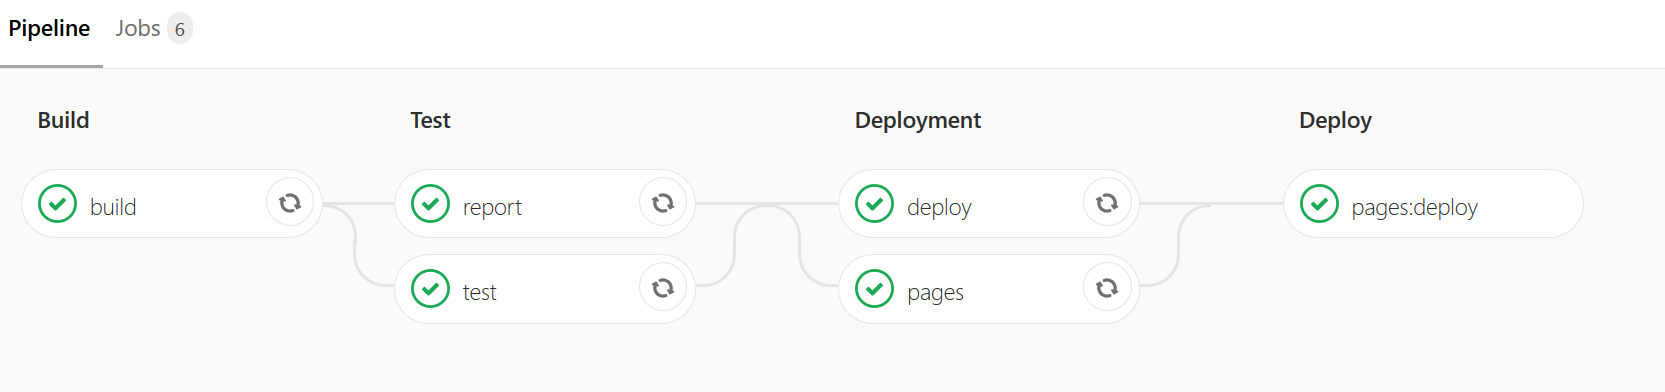
\includegraphics[width=0.9\textwidth]{M5_Pipeline}
 	\caption{Pipeline de GitLab que muestra éxito en todos los trabajos definidos para el proceso de CI/CD}\label{fig:M5_Pipeline}
 \end{figure}
 \FloatBarrier
 
 
 En la Fig. \ref{fig:M5_Pipeline_Error} se muestra un pipeline que dió error en la actividad de \textit{report} y, en consecuencia, se pasó por alto la actividad \textit{deploy}.
 
 \imagen{M5_Pipeline_Error}{Error en un pipeline}
%\todo añadir una captura de pantalla con el badge Heroku del  Readme de Gitlab y explicar como se actualiza cada vez que se realiza un commit. 
%\todo añadir una captura de pantalla con los check verdes en la lista de commit del repositorio de GitLab

\subsubsection{Tokens y variables de entorno}

Para llevar a cabo este proceso de CI/CD, ha sido necesario definir variables de entorno en GitLab que contienen las credenciales o tokens de acceso a Heroku y a Codacy. Esto se realiza desde la ventana de Configuración-CI/CD en la parte de `\textit{Variables}' como se muestra en la Fig. \ref{fig:M5_GitLab_Variables}.

\imagen{M5_GitLab_Variables}{Variables del entorno de ejecución de GitLab}

En el apartado anterior se vé un fragmento de código en el que se utilizan dos de las tres variables que se han definido y se ven en la Fig. \ref{fig:M5_GitLab_Variables}: \ruta{\$CODACY\_PROJECT\_TOKEN} y \ruta{\$CODACY\_API\_TOKEN}. La otra variable (\ruta{HEROKU\_API\_KEY}) se utiliza indirectamente en la actividad de \textit{deploy} de la etapa de \textit{deployment}. Esta no se muestra en el script que define la actividad, sin embargo, fallaría la ejecución de la actividad si no se hubiera definido esta variable.

Estos tokens permiten conectarse a herramientas como Codacy o Heroku ya sea para iniciar sesión o para acceder directamente a un proyecto definido dentro de esas herramientas sin necesidad de tener que tener que iniciar sesión manualmente mediante usuario y contraseña. Esto permite automatizar las tareas que requieran iniciar sesión en herramientas de este tipo. Por ejemplo, \ruta{\$CODACY\_PROJECT\_TOKEN} es el token que da acceso al proyecto correspondiente en Codacy y \ruta{\$CODACY\_API\_TOKEN} permite utilizar Codacy con una sesión de usuario sin tener que iniciar sesión manualmente. Estos tokens se han obtenido de Codacy: \ruta{\$CODACY\_PROJECT\_TOKEN} se obtuvo al configurar la cobertura de código en Codacy y \ruta{\$CODACY\_API\_TOKEN} desde la configuración de la cuenta de usuario en Codacy, en la pestaña `\textit{API Tokens}'.

\subsubsection{Badges}

Los badges son distintivos que se añaden en el fichero \ruta{README} o en el lugar que se permita (admiten varios formatos como Markdown, HTML, Textile, AciiDoc, etc) y aportan información sobre el estado de ciertas características del proyecto tras el último commit como el resultado del pipeline de una actividad de CI/CD, la revisión de calidad, la revisión de cobertura, el estado del despliegue, etc.

En la Fig. \ref{fig:M5_GitLab_Badges_Readme} se muestran los badges que se han definido en el fichero \ruta{README.md} del proyecto. Los badges constan de tres partes:
\begin{itemize}
	\tightlist
	\item Nombre del badge
	\item Imagen en formato \textit{.svg} asociada al estado del atributo que evalúa el badge y ofrecida por el proveedor de la información
	\item Enlace a una página que complete la información que ofrece el badge.
\end{itemize}

En Markdown la sintaxis es la siguiente:\\
\begin{minipage}{\linewidth}
{\tiny
\begin{lstlisting}[breaklines]
[![nombre-del-badge](URL-de-la-imagen)](URL-del-link)
\end{lstlisting}
}
\end{minipage}
mientras que en HTML sería:\\
\begin{minipage}{\linewidth}
{\tiny
\begin{lstlisting}[breaklines]
<a href="URL-del-link"><img src="URL-de-la-imagen"/></a>
\end{lstlisting}
}
\end{minipage}

\imagen{M5_GitLab_Badges_Readme}{Badges definidas en el fichero README.md del repositorio del proyecto}

En el proyecto se han definido cuatro badges:
\begin{itemize}
	\item \textit{\textbf{Pipeline}}. Muestra la información del último \textit{pipeline} del proyecto ejecutado en GitLab: en ejecucion (\textit{running}), ejecutado correctamente (\textit{passed}), o ejecutado con fallos (\textit{failed}). El proveedor de la imagen y de la información es GitLab y enlaza con el último \textit{pipeline} del proyecto.
	
	\item \textit{\textbf{Code Quality}}. Muestra la calificación de calidad de código que da Codacy al proyecto y enlaza a la página del proyecto en Codacy.
	
	\item \textit{\textbf{Coverage}}. Muestra el porcentaje de cobertura de instrucciones de las pruebas que se realizan durante la ejecución del \textit{pipeline} de GitLab y enlaza a la página del proyecto en Codacy. El dato es recogido durante la actividad \textit{report} de la fase de \textit{test} del \textit{pipeline}.
	
	\item \textit{\textbf{Coverage}}. Debido a problemas con Codacy, se ha decidido poner otro badge de cobertura. Esta vez se obtiene la información directamente desde el pipeline del último commit del repositorio del proyecto. Y enlaza a un informe que genera JaCoCo en formato HTML y que es publicado en el mismo repositorio del proyecto.
\end{itemize}

\subsection{Pruebas unitarias automáticas con JUnit y GitLab}

Para la automatización de la fase de pruebas se han utilizado las herramientas JUnit, Maven y los \textit{pipelines} GitLab.

\subsubsection{Desarrollo de las pruebas con JUnit}

JUnit es un framework que permite desarrollar pruebas unitarias sobre el código desarrollado. Además, dispone de un motor para la ejecución de las pruebas y la visualización de los resultados. En este proyecto se ha utilizado JUnit 5. Esta es la última versión de JUnit y permite, entre otras cosas:
\begin{itemize}
	\item Realizar asertos (\textit{asserts}) de tipo \textit{\textbf{assertAll()}} \footnote{\url{https://junit.org/junit5/docs/current/api/org/junit/jupiter/api/Assertions.html}}. Este tipo de asertos permite tratar varios asertos como una unidad. Se utilizaron en versiones anteriores de la aplicación, pero realmente no eran necesarios y se optó por quitarlos.
	
	\item Realizar \textbf{comprobaciones de lanzamiento de excepciones} en asertos del tipo \textit{assertThrows()}. De esta forma se pueden comprobar todos los casos de pruebas, tanto aquellos en los que se espere un resultado como aquellos en los que se debería lanzar una excepción. Por ejemplo, un test que espera una excepción sería:\\
\begin{minipage}{\linewidth}
{\tiny
\begin{lstlisting}[breaklines]
...
@ParameterizedTest(name = "Run with User = \"{0}\" and Password = \"{1}\" must throw an exception.")
@CsvFileSource(resources = "/testConnectUserPasswordWrong.csv", numLinesToSkip = 1, delimiter = ';', encoding = "UTF-8")
public void testConnectUserPasswordWrong(String user, String password) {
  assertThrows(RepositoryDataSourceException.class, () -> {
	repositoryDataSource.connect(user, password);
  }, getErrorMsg("testConnectUserPasswordWrong", "Wrong user-password should throw an exception"));
  assertEquals(EnumConnectionType.NOT_CONNECTED, repositoryDataSource.getConnectionType(), getErrorMsg("testConnectUserPasswordWrong", "Connection type must be 'NOT_CONNECTED'"));
}
...		
\end{lstlisting}
}
\end{minipage}
	
	Este comprueba que tras ejecutar la función con un conjunto de combinaciones posibles de usuario y contraseña incorrectos como argumentos, se lance una excepción y se mantenga un estado consistente en un objeto de la clase \textit{RepositoryDataSource}.
	
	\item Permite crear \textbf{test parametrizados} para probar funciones que requieren argumentos.
	
	Hay que tener en cuenta que cada combinación de estos argumentos es un caso de prueba. Crear un test para cada combinación de argumentos es un caso claro del defecto de código `código duplicado' y dificultan la mantenibilidad del proyecto. Por ello estos argumentos se pueden generar mediante funciones, enumeraciones, proveedores de argumentos o recolectar desde un \textit{CSV} y solo ser necesario un test para todas las combinaciones de argumentos posibles. Otra ventaja de poder realizar pruebas parametrizadas es que el mismo \textit{CSV} sirve para diferentes funciones de pruebas.
	
	Para poder parametrizar los test es necesario agregar una dependencia adicional al proyecto \ruta{junit-jupiter-params} junto con la dependencia del API de JUnit \ruta{junit-jupiter-api}.
	
	Un ejemplo de estos se encuentra en el código anterior, que tiene la anotación \ruta{@ParameterizedTest} y recibe los argumentos de un fichero \textit{CSV} ubicado en \ruta{src/test/resources} llamado \ruta{testConnectUserPasswordWrong.csv}, que contiene los datos de prueba:\\
\begin{minipage}{\linewidth}
{\tiny
\begin{lstlisting}[breaklines]
USER;PASSWORD
;a
a;
;
"";a
a;""
"";""
mlb0029;a	
\end{lstlisting}
}
\end{minipage}
	
	Cada columna del CSV es un argumento de la función. La diferencia entre poner comillas dobles y no poner nada es escribir un \textit{String} vacío o \textit{null}, respectivamente. La primera linea es la cabecera para mejorar la comprensión del \textit{CSV}. Para no contar esa linea como argumentos, se debe configurar la anotación \textit{@CsvFileSource} con 
\begin{minipage}{\linewidth}
{\tiny
\begin{lstlisting}[breaklines]
numLinesToSkip = 1
\end{lstlisting}
}
\end{minipage} 
como se puede observar en el código del punto anterior.
		
	\item Permite realizar presunciones (\textit{\textbf{assumptions}}) que pasarán por alto el test sin marcarla como error (lo marca como \textit{skipped}) en caso de que no se cumpla una condición. 
	
	Esto ha sido útil de cara a probar funciones que realicen conexiones a GitLab que requieran credenciales de acceso. No es correcto escribir en el código las credenciales de acceso, por tanto estos test tienen presunciones que comprueban que se tienen las credenciales de acceso (p.ej en un fichero o en variables auxiliares). En tiempo de desarrollo se proporcionan las credenciales, mientras que en el proceso de integración continua de GitLab, no se proporcionan de ninguna manera. Sin embargo, en lugar de lanzar un error por no tener las credenciales, los test se pasan por alto y no se ejecutan.
\end{itemize}

\subsubsection{Proyectos de pruebas}

Para realizar pruebas en la obtención de información de repositorios de GitLab se han creado dos proyectos de pruebas (uno privado y otro público) y se ha utilizado otro adicional importado desde GitHub de uno de los trabajos para una asignatura:
\begin{itemize}
	\tightlist
	\item \url{https://gitlab.com/mlb0029/privatetestproject}
	\item \url{https://gitlab.com/mlb0029/publictestproject}
	\item \url{https://gitlab.com/mlb0029/ListaCompra}
\end{itemize}
Se han realizado commits e issues en los proyectos que se han creado para probar las funciones que obtienen información de GitLab. Estos datos se han almacenado en ficheros \textit{CSV} para poder parametrizar las pruebas (ver Fig. \ref{fig:M5_CSV_ProyectosPruebas}).

\imagen{M5_CSV_ProyectosPruebas}{Datos de proyectos de pruebas en fichero CSV}

Aunque no para las pruebas automáticas, también ha sido posible probar la aplicación con datos de otros repositorios de GitLab que se han presentado como TFG en el Grado de Ingeniería Informática en la Universidad de Burgos. Es destacable la funcionalidad de acceso a los repositorios por el concepto de grupo definido en GitLab. Esto fue posible gracias a que la empresa Hewlett Packard SCDS en su colaboración con TFGs con la UBU organiza sus propuestas de TFGs en GitLab en grupos para organizarlos por cursos académicos.

\subsubsection{Automatización de las pruebas}

Para automatizar el proceso de pruebas se ha utilizado Maven y los \textit{pipelines} de GitLab.

Para ello se debe incluir una dependencia al proyecto: \ruta{junit-jupiter-engine} que es el motor de ejecución de pruebas de JUnit y en el \ruta{build} incluir los siguientes plugins:\\
\begin{minipage}{\linewidth}
{\tiny
\begin{lstlisting}[breaklines]
  <!-- Unit tests -->
  <plugin>
	<groupId>org.apache.maven.plugins</groupId>
	<artifactId>maven-surefire-plugin</artifactId>
	<configuration>
	  <reportsDirectory>${project.reporting.outputDirectory}/surefire-reports</reportsDirectory>
	</configuration>
	<version>2.22.1</version>
  </plugin>
  <!-- Integration tests -->
  <plugin>
	<groupId>org.apache.maven.plugins</groupId>
	<artifactId>maven-failsafe-plugin</artifactId>
	<version>2.22.1</version>
  </plugin>	
\end{lstlisting}
}
\end{minipage}

Con esto, se puede ejecutar \textit{mvn test} para ejecutar las pruebas. Este comando puede ser agregado en una de las actividades del fichero \ruta{.gitlab-ci.yml} para ejecutar las pruebas automáticamente al hacer un commit en GitLab. Por ejemplo, la actividad \textit{test} de la fase \textit{test}:\\
\begin{minipage}{\linewidth}
{\tiny
\begin{lstlisting}[breaklines]
...
test:
  stage: test
  script:
	- mvn test
...
\end{lstlisting}
}
\end{minipage}

\subsection{Pruebas con Tomcat}

Desde que se empezó ha implementar la interfaz se configuró un entorno Tomcat en el que poder desplegar la aplicación y visualizar y probar los elementos de la interfaz gráfica.

Para realizarlo se instaló Tomcat en el equipo local del programador y se configuró la correspondiente variable de entorno del sistema \ruta{CATALINA\_HOME} con la ruta a la carpeta de instalación. Conviene, también, tener definida la variable \ruta{JAVA\_HOME} apuntando al directorio de instalación del JDK o del JRE de Java.

Como \textit{Eclipse IDE for Java EE Developers} y Tomcat se integran muy bien, se puede configurar un servidor Tomcat con Eclipse desde la vista \textit{Servers}. Solo hay que elegir la versión de Tomcat (la 9 para Java 11) y especificar: el nombre del servidor, el directorio de instalación de Tomcat y el JRE a utilizar (Java 11). Una vez hecho esto se puede desplegar la aplicación desde eclipse fácilmente (\textit{Run As/Run on Server}), siempre que el puerto 8080 que usa Tomcat esté disponible y el servidor arrancado. Se puede acceder a la aplicación desde el navegador con la url: \ruta{http://localhost:8080/[nombre-proyecto]} y probar la aplicación en distintos navegadores.

También se puede hacer sin Eclipse. Para ello, solo basta con tener el puerto 8080 disponible y ejecutar en una consola de comandos el comando \textit{startup}. Se arrancará el servidor Tomcat, pero antes conviene configurar un usuario de Tomcat con rol `\textit{manager-gui}' desde el fichero \ruta{\$CATALINA\_HOME/conf/tomcat-users.xml}. Por ejemplo:\\
\begin{minipage}{\linewidth}
{\tiny
\begin{lstlisting}[breaklines]
...
<role rolename="manager-gui"/>
<user username="blah" password="blah" roles="manager-gui"/>
...
</tomcat-users>
\end{lstlisting}
}
\end{minipage}
Una vez arrancado Tomcat, se puede acceder desde el navegador a \ruta{http://localhost:8080} (aparecerá una ventana similar a la de la Fig. \ref{fig:M5_Tomcat_Main}) y pulsar sobre \textit{Manager App}. Desde el gestor de aplicaciones se pueden desplegar varias aplicaciones, publicando el fichero \ruta{.war} de la aplicación.

\imagen{M5_Tomcat_Main}{Ventana principal de la GUI de Tomcat}

Cada vez que se añadía un elemento a la interfaz se realizaban pruebas y se cuadraba el elemento dentro de la interfaz. Una vez que se creaba una funcionalidad completa, también se realizaban pruebas sobre la interfaz. Por ejemplo, añadir un repositorio o calcular las métricas.

\subsection{Revisión automática de la cobertura con Codacy}

La cobertura es el porcentaje de la aplicación que se ha probado. Esto se puede medir en relación a lineas de código, instrucciones, clases, bifurcaciones (condicionales y bucles) y métodos. Lo normal es mostrar la cobertura de instrucciones.

Para realizar las revisiones automáticas de cobertura, lo primero que hay que hacer es definir las pruebas y ejecutarlas. Como este proceso se ha explicado anteriormente, se procede a describir el proceso de cobertura.

Las revisiones automáticas de cobertura se han realizado utilizando JaCoCo, Codacy y GitLab. Sin embargo, JaCoCo es el que genera los informes que se envían tanto a Codacy como a GitLab.

\subsubsection{Configuración de JaCoCo con Maven}

Antes que nada se ha añadido una sección en el fichero \ruta{pom.xml}:\\
\begin{minipage}{\linewidth}
{\tiny
\begin{lstlisting}[breaklines]
...
<reporting>
  <outputDirectory>${project.build.directory}/reports</outputDirectory>
</reporting>
...
\end{lstlisting}
}
\end{minipage}
en la que se define el directorio donde se generarán todos los informes (incluidos los informes de las pruebas). Y en la sección de \textit{build} se añade el siguiente plugin de la siguiente manera:\\
\begin{minipage}{\linewidth}
{\tiny
\begin{lstlisting}[breaklines]
...
<plugin>
  <groupId>org.jacoco</groupId>
  <artifactId>jacoco-maven-plugin</artifactId>
  <version>0.8.3</version>
  <configuration>
	<outputDirectory>${project.reporting.outputDirectory}/jacoco-reports</outputDirectory>
	<output>file</output>
	<title>Coverage of project: ${project.name}</title>
  </configuration>
</plugin>
...
\end{lstlisting}
}
\end{minipage}
En la configuración se define:
\begin{itemize}
	\tightlist
	\item El directorio de destino de los informes
	\item Que se desea que se generen en forma de fichero
	\item El título del fichero
\end{itemize}
 De esta forma, se puede generar los informes con Maven de la siguiente manera:\\
\begin{minipage}{\linewidth}
{\tiny
\begin{lstlisting}[breaklines]
$ mvn clean jacoco:prepare-agent install jacoco:report
$ mvn jacoco:report
\end{lstlisting}
}
\end{minipage}

El primer comando genera el fichero \ruta{jacoco.exec} que es necesario para la ejecución del segundo comando.

\subsubsection{Configuración de Codacy}

Codacy permite llevar una revisión de la calidad de código y de la cobertura de las pruebas.

Para utilizar esta herramienta se debe tener una cuenta. Permite iniciar sesión con GitHub, Bitbucket o Google. Una vez iniciada sesión permite añadir proyectos al entorno Codacy. Para añadir proyectos se debe pulsar sobre el botón \textit{Add project} como se muestra en la Fig. \ref{fig:M5_Codacy_ProjectsPage}. Se pueden importar los proyectos desde GitHub o Bitbucket (hay que solicitar permisos a GitHub o Bitbucket). Nada más añadirlos, realiza un análisis inicial de la calidad de código y, posteriormente, realizará este análisis cada vez que se realice un \textit{commit} en GitHub o Bitbucket.

\imagen{M5_Codacy_ProjectsPage}{Página principal de Codacy para la gestión de proyectos}

Para configurar la revisión de cobertura hay que seguir unos pasos más. Desde la página de \textit{Dashboard} del proyecto (ver Fig. \ref{fig:M5_Codacy_Dashboard}) se puede observar el indicador de cobertura con título \textit{Coverage}. En un proyecto nuevo, este indicador no está disponible hasta que se haya configurado la cobertura, en su lugar aparece el siguiente mensaje: ``\textit{Make sure your code is all tested. Set up your coverage here.}'' con un enlace. El enlace lleva a una página que contiene el token del proyecto e instrucciones a seguir según el lenguaje de programación.

\imagen{M5_Codacy_Dashboard}{Vista Dashboard del proyecto en Codacy}

Para este proyecto, la configuración de cobertura de Codacy se ha realizado de la siguiente manera:
\begin{enumerate}
	\item Copiar en algún fichero o en el portapapeles el token del proyecto que se muestra en la página de instrucciones mencionada anteriormente (importante).
	
	\item Configurar el plugin JaCoCo como se ha indicado anteriormente.
	
	\item Utilizar \textit{codacy-maven-plugin} para enviar el informe de cobertura generado por JaCoCo a Codacy. También se puede añadir el plugin en la sección de \textit{buid} del \ruta{pom.xml}:\\
\begin{minipage}{\linewidth}
{\tiny
\begin{lstlisting}[breaklines]
<plugin>
  <groupId>com.gavinmogan</groupId>
  <artifactId>codacy-maven-plugin</artifactId>
  <version>1.2.0</version>
  <configuration>
	<coverageReportFile>${project.reporting.outputDirectory}/jacoco-reports/jacoco.xml</coverageReportFile>
  </configuration>
</plugin>
\end{lstlisting}
}
\end{minipage}
	En la configuración se le indica la ubicación del fichero que debe enviar a Codacy.

	\item Para enviar el informe de cobertura se tendrá que generar los informes de JaCoCo con los comandos Maven del apartado anterior y ejecutar el siguiente comando:\\
\begin{minipage}{\linewidth}
{\tiny
\begin{lstlisting}[breaklines]
$ mvn com.gavinmogan:codacy-maven-plugin:coverage -DprojectToken="$CODACY_PROJECT_TOKEN" -DapiToken="$CODACY_API_TOKEN"
\end{lstlisting}
}
\end{minipage}
	Siendo \ruta{\$CODACY\_PROJECT\_TOKEN} el token del proyecto del que se habla en el primer punto y \ruta{\$CODACY\_API\_TOKEN} el token de usuario para utilizar el API de Codacy. Este último se obtiene desde la gestión de la cuenta de usuario.
\end{enumerate}

\subsubsection{Configuración de GitLab}

Se ha configurado JaCoCo y el plugin para enviar los informes de JaCoCo a Codacy para realizar estas actividades con comandos Maven. Pero para automatizar este proceso se deben añadir las actividades correspondientes al flujo de trabajo de CI/CD de GitLab, es decir: el fichero \ruta{.gitlab-ci.yml}.

Para ello se ha definido la actividad \textit{report} en la etapa de \textit{test}, ejecutando los comandos Maven  con unas pequeñas modificaciones:\\
\begin{minipage}{\linewidth}
{\tiny
\begin{lstlisting}[breaklines]
report:
  stage: test
  script:
	- mvn clean jacoco:prepare-agent install jacoco:report
	- mvn jacoco:report -DdataFile=$CI_PROJECT_DIR/target/jacoco.exec
	- mvn com.gavinmogan:codacy-maven-plugin:coverage -DprojectToken="$CODACY_PROJECT_TOKEN" -DapiToken="$CODACY_API_TOKEN"
  artifacts:
	paths:
	  - $CI_PROJECT_DIR/target/reports/jacoco-reports/
\end{lstlisting}
}
\end{minipage}
\begin{itemize}
	\item En el segundo comando se añade la opción \ruta{-DdataFile} que indica la ubicación del fichero \ruta{jacoco.exec} que se genera en el entorno de GitLab.
	\item Para utilizar \ruta{\$CODACY\_PROJECT\_TOKEN} y \ruta{\$CODACY\_API\_TOKEN} se deben configurar las variables de entorno de GitLab como se indica en la sección `Tokens y variables de entorno'.
	\item Se ha añadido \textit{artifacts} con la ruta que apunta al directorio que contiene los informes de JaCoCo definido en Maven (ver `Configuración de JaCoCo con Maven'). Con esto se agrega este directorio a los artefactos de la actividad.
\end{itemize}

La parte de \textit{artifacts} no tiene que ver con JaCoCo ni con Codacy. Entonces, ¿por qué añadirlo? 

Codacy tenía demasiados problemas al soportar GitLab y otras forjas de repositorios (añadir proyecto a Codacy con \textit{Git URL}) y decidieron eliminar esta funcionalidad. Por tanto, cesaron las revisiones automáticas de calidad y cobertura. Para solucionar esto se puede exportar a GitHub el proyecto y añadir el proyecto a Codacy impostándolo desde GitHub. Sin embargo, se deseaba seguir trabajando con GitLab. Una solución es hacer un \textit{Git push} tanto para GitLab como para GitHub cada vez que se realice un commit y en GitLab añadir los badges y las variables de entorno que enlazan al proyecto en Codacy, pero que realmente es importado desde GitHub.

Adicionalmente, se estudió la forma de agregar la cobertura directamente desde GitLab. Se encontró que es posible publicar directamente el informe de JaCoCO en formato \textit{HTML} en GitLab y añadir un badge de Cobertura. Para ello, se debe generar el informe con formato HTML en una de las actividades y almacenarlo en los artefactos de la actividad. Esta es la explicación de \textit{artifacts}. Posteriormente se publican estos artefactos en las páginas del proyecto en GitLab (\ruta{Settings - Pages}). Lo mejor sería añadir el enlace al informe en el fichero \ruta{README} del proyecto y ¿qué mejor forma que añadirlo en forma de badge?. 

Para agregar el badge se necesita mostrar en un log de las actividades un informe de cobertura donde venga el porcentaje total: el fichero \ruta{index.html} generado por JaCoCO tiene este dato. Lo que falta es añadir la expresión regular que lo identifica en el fichero en la configuración del proyecto (\ruta{Settings - CI/CD -  General pipelines}) en la parte de `Test coverage parsing'. La expresión regular es la siguiente para ese fichero:\\
\begin{minipage}{\linewidth}
{\tiny
\begin{lstlisting}[breaklines]
/<td>Total<\/td><td class="bar">\d{1,3}(,\d{1,3})? of \d{1,3}(,\d{1,3})?<\/td><td class="ctr2">(\d{1,3})%<\/td>/
\end{lstlisting}
}
\end{minipage}
Si se muestra el informe en el log de las actividades de un \textit{pipeline}, y se ha definido bien la expresión regular, desde \ruta{Settings - CI/CD -  General pipelines} se muestran tanto el badge del estado del \textit{pipeline} como el de cobertura (ver Fig. \ref{fig:M5_GitLab_Badges_CoverageAndPipeline}). Solo queda añadirlos al fichero \ruta{README} y/o a los badges del proyecto como se indica en la sección `Badges'. Se recomienda cambiar el enlace del badge del informe de cobertura por el enlace al informe de cobertura de JaCoCO publicado en las \ruta{Pages} del proyecto.

\imagen{M5_GitLab_Badges_CoverageAndPipeline}{Configuración de CI/CD de GitLab: Pipeline status and Coverage report}

La publicación del informe y mostrar en el log el fichero \ruta{index.html} se realiza en la actividad \textit{pages} de la fase \textit{deployment} de la siguiente manera:\\
\begin{minipage}{\linewidth}
{\tiny
\begin{lstlisting}[breaklines]
...
pages:
  stage: deployment
  dependencies: 
	- report
  script:
	- cat $CI_PROJECT_DIR/target/reports/jacoco-reports/index.html
	- mv $CI_PROJECT_DIR/target/reports/jacoco-reports/ public/
  artifacts:
	paths:
	  - public
	expire_in: 30 days    
  only:
	- master
...
\end{lstlisting}
}
\end{minipage}

Con el comando \ruta{cat} se visualiza en el log el fichero \ruta{index.html} y con el comando \ruta{mv} de publican los documentos HTML del informe de cobertura. También se almacenan los artefactos del directorio \textit{public} en el \textit{pipeline} durante 30 días. Y se ha configurado para que la actividad solo se ejecute al realizar cambios en la rama \ruta{master} si la actividad \textit{report} se ha ejecutado sin problemas.

\subsection{Administración de calidad automática con Codacy}

Ya se ha mencionado en la sección `Configuración de Codacy' que este realiza revisiones automáticas de calidad y cómo se configura para ello, siendo un proceso bastante sencillo. Esto permite analizar la deuda técnica y, en caso de ser necesario, definir tareas para disminuir dicha deuda. 

La valoración final del proyecto ha sido la máxima (A), se muestra en el badge de `Code Quality' como se puede ver en la Fig. \ref{fig:M5_GitLab_Badges_Readme}. Al pulsar sobre el badge se abre una pestaña en el navegador redirigida al proyecto en Codacy (\url{https://app.codacy.com/manual/mlb0029/comparador-de-metricas-de-evolucion-en-repositorios-software/dashboard}), como se muestra en la Fig. \ref{fig:M5_Codacy_Dashboard_Complete}.

\imagen{M5_Codacy_Dashboard_Complete}{Dashboard del proyecto en Codacy}

Este muestra la evolución en el tiempo de la deuda técnica y una vista del estado actual de: el porcentaje de problemas de calidad (4\%), la complejidad de los ficheros (0\%), el código duplicado (0\%) y la cobertura (si se ha configurado) (18\%). Este gráfico ha ayudado a lo largo del desarrollo de la aplicación a valorar la evolución de la deuda técnica. En momentos de crecimiento, se puede ir a la ventana `Issues'  y ver los defectos de diseño que causan el aumento de la deuda (ver Fig. \ref{fig:M5_Codacy_Issues}). Se muestran los problemas por fichero y se muestra la linea de código que se debe corregir para disminuir la deuda técnica.

\begin{figure}[!h]
	\centering
	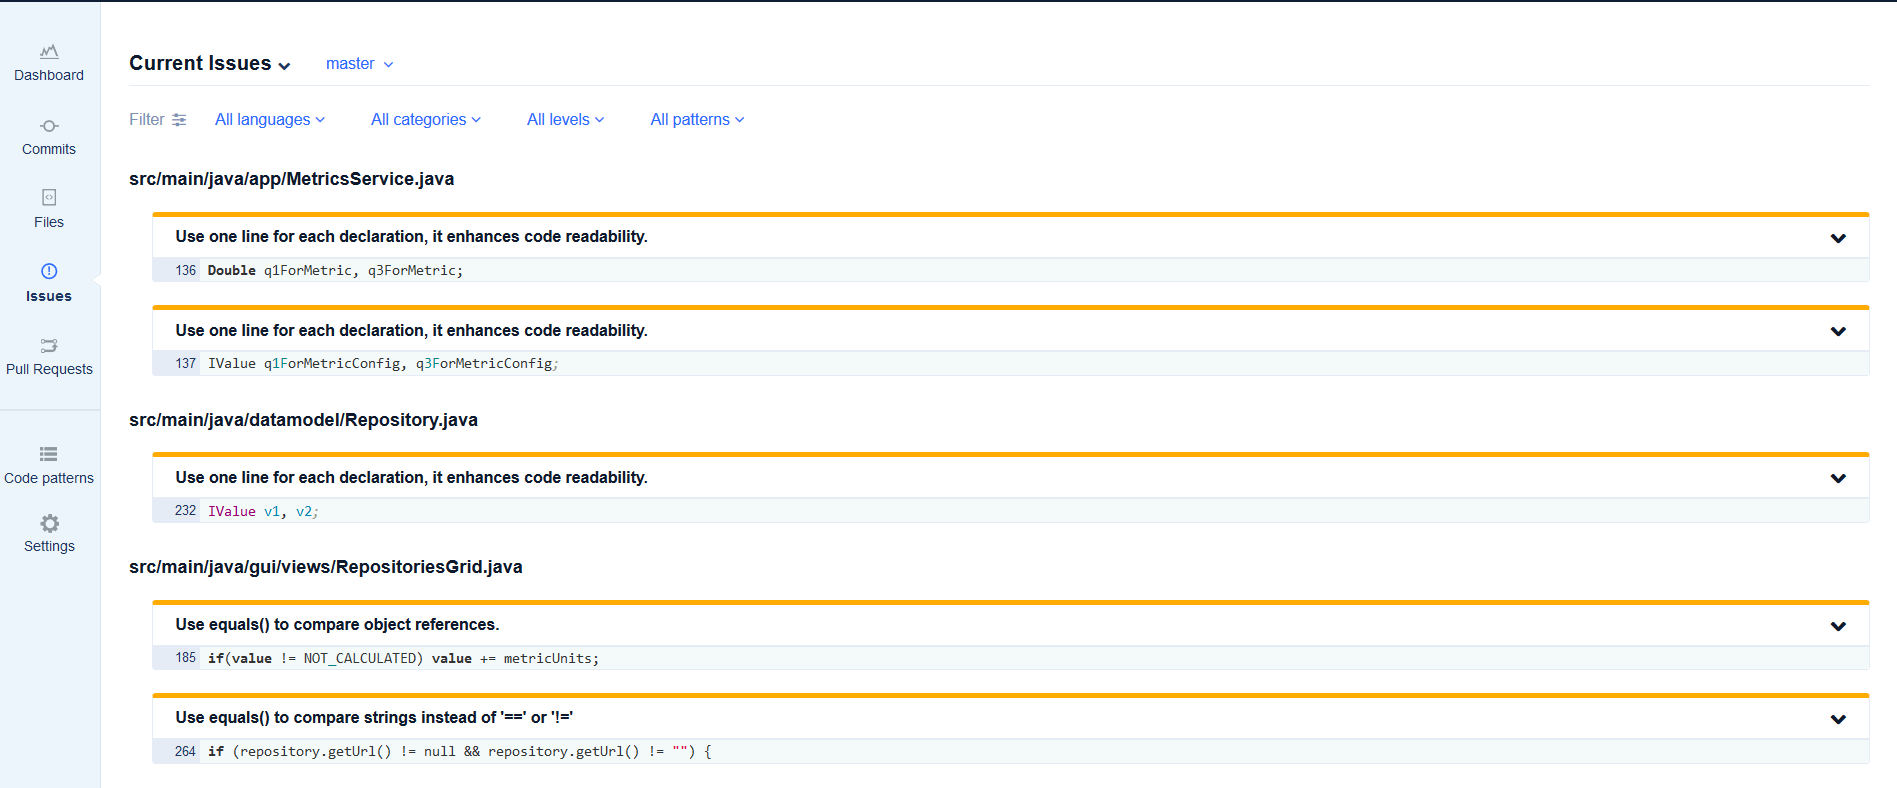
\includegraphics[width=1.0\textwidth]{M5_Codacy_Issues}
	\caption{Ventana Issues de Codacy con defectos que causan aumento de la deuda técnica}\label{fig:M5_Codacy_Issues}
\end{figure}
\FloatBarrier

Al gestionar la revisión de calidad por primera vez en este proyecto, Codacy permitía añadir repositorios a partir de su \textit{Git URL}. Esto permitió añadir nuestro proyecto de GitLab al entorno de Codacy. Sin embargo, esta funcionalidad les daba muchos problemas y la acabaron eliminando. Esto paró las revisiones de calidad automáticas de este proyecto. Para solucionar este problema se ha exportado el proyecto a GitHub, se ha puesto este como repositorio remoto secundario y se ha añadido a Codacy para realizar una revisión final, con el código ya creado. En la Fig. \ref{fig:M5_Codacy_Dashboard_Complete} no se aprecia el gráfico de evolución, debido a que no se han realizado apenas revisiones de calidad. Sin embargo, en la figura \ref{fig:M3_Codacy} se muestra una captura realizada antes de este incidente y se puede apreciar ese gráfico.

\subsection{Despliegue automático con Heroku}

\subsubsection{Configuración de la Herramienta Heroku}

Heroku es una plataforma que permite desplegar una aplicación Web en sus servidores. Para ello debes tener una cuenta, crear un pipeline y una aplicación y asociar la aplicación al pipeline. Para desplegarla se ofrecen tres opciones: \textit{Heroku Git}, \textit{GitHub} y \textit{Heroku CLI}.

En este proyecto se ha utilizado Heroku CLI y un plugin para integrarlo con Maven:\\
\begin{minipage}{\linewidth}
{\tiny
\begin{lstlisting}[breaklines]
...
<plugin>
  <groupId>com.heroku.sdk</groupId>
  <artifactId>heroku-maven-plugin</artifactId>
  <version>2.0.9</version>
  <configuration>
	<appName>evolution-metrics</appName>
  </configuration>
</plugin>
...
\end{lstlisting}
}
\end{minipage}

En el código anterior se configura el plugin para desplegar en la aplicación con nombre \textit{evolution-metrics}. El comando para  desplegar la aplicación sería \ruta{\$ mvn clean heroku:deploy-war}. Sin embargo, para que funcione correctamente se debe iniciar sesión con \ruta{\$ heroku login}, que abre el navegador en la página de inicio de sesión de Heroku. De esta forma es imposible desplegar la aplicación automáticamente, para hacerlo se debe configurar la variable de entorno \ruta{HEROKU\_API\_KEY} con el token de acceso \textit{API Key} que se obtiene desde la configuración de la cuenta de usuario de Heroku. Esta variable se ha definido dentro de las variables de entorno de GitLab de las que se hablaba anteriormente, y el comando de despliegue se ejecuta desde los \textit{pipelines} gracias a la actividad \textit{deploy} de la etapa \textit{deployment} definidas en el fichero \ruta{.gitlab-ci.yml}.

\section{API de GitLab}

GitLab ofrece un API \footnote{\url{https://docs.gitlab.com/ee/api/}} REST \footnote{Representational state transfer} para poder desarrollar aplicaciones que integren funcionalidades de GitLab. En este proyecto se ha utilizado este API para establecer una conexión a GitLab y poder calcular métricas de los repositorios que aloje. Sin embargo, en lugar de trabajar directamente con GitLab REST API, se decidió usar un API en Java que permita operar con las características de GitLab REST API desde Java. Se encontraron dos proyectos en GitHub que implementan este tipo de APIs:
\begin{itemize}
	\tightlist
	\item \textit{timols/java-gitlab-api} \footnote{\url{https://github.com/timols/java-gitlab-api}}. 
	\item  \textit{gitlab4j/gitlab4j-api} \footnote{\url{https://github.com/gitlab4j/gitlab4j-api}}.
\end{itemize}

La primera impresión al entrar en \textit{timols/java-gitlab-api} es que el fichero \ruta{README} está bastante vacío, tan solo contiene una descripción de lo que es y un enlace a la documentación. Al entrar en la documentación se puede observar que el código no está muy bien documentado, faltan muchas descripciones de funciones. Por estas razones, el coste de aprendizaje del API es muy alto y casi incomprensible. Además, tiene bastantes \textit{issues} abiertas y la última \textit{release} es de octubre de 2018, por lo que parece que la evolución del proyecto es lenta o a cesado.

Por el lado contrario, \textit{gitlab4j/gitlab4j-api} tiene un fichero \ruta{README} explicativo, con índice de contenidos y muchos ejemplos. La documentación también tiene muchos elementos sin comentar, pero si que se ha documentado gran parte del sistema. El proyecto tiene muy pocas issues abiertas y está en constante evolución, sacando tres o cuatro \textit{releases} al mes y evolucionando a la vez que GitLab REST API. Es por estos factores por los que se decidió usar este API como intermediario entre nuestra aplicación en Java y GitLab REST API, y para ello, solo ha sido necesario incluirlo entre las dependencias del proyecto en el fichero \ruta{pom.xml}. 

\section{Diseño extensible}

En la sección \ref{sect:3_3_3_FrameworkMedicion} - `Framework de medición' se detalla como se implementa un framework de medición que permite la reutilización en el cálculo de métricas. Esto permite implementar nuevas métricas sin complejidad alguna.

Además, el paquete \textit{repositorydatasource}, que realiza la conexión con GitLab, se ha creado de forma que se facilite la extensión a otras forjas de repositorios como GitHub o Bitbucket. De esta forma solo hace falta implementar las dos interfaces que se definen en el paquete: \textit{RepositoryDataSource} y \textit{RepositoryDataSourceFactory} (aplicación del patrón de diseño: método fábrica). Esto ha sido probado por el tutor de este TFG y ha conseguido terminar la funcionalidad en una semana. La implementación se encuentra en una nueva rama del proyecto \footnote{\url{https://gitlab.com/mlb0029/comparador-de-metricas-de-evolucion-en-repositorios-software/tree/github}}. La complejidad reside en encontrar un API de conexión a GitHub y utilizarlo para obtener las métricas. Una linea de trabajo futura sería unir las dos ramas y hacer cambios en la interfaz gráfica para que soporte tanto GitLab como GitHub.

También se han añadido pequeños puntos de extensión en la interfaz gráfica para implementar nuevas formas de conexión y de añadir repositorios. 

Para implementar nuevas formas de añadir repositorios solo bastaría con implementar la clase abstracta \textit{AddRepositoryFormTemplate} y agregar una nueva linea en la función:\\
\begin{minipage}{\linewidth}
{\tiny
\begin{lstlisting}[breaklines]
...
private void createConnectionForms() {
  addRepositoryForms.add(new AddRepositoryFormByUsername());
  addRepositoryForms.add(new AddRepositoryFormByGroup());
  addRepositoryForms.add(new AddRepositoryFormByURL());
}
...
\end{lstlisting}
}
\end{minipage}
 de la clase \textit{AddRepositoryDialog} que llame al constructor de la clase implementada.
 
 Para implementar nuevas formas de conexión (serviría para agregar una funcionalidad que cambie el \textit{RepositoryDataSource} de GitLab a GitHub) bastaría con implementar la clase abstracta \textit{ConnectionFormTemplate} o directamente la interfaz \textit{ConnectionForm} y agregar una nueva linea en la función:\\
\begin{minipage}{\linewidth}
{\tiny
\begin{lstlisting}[breaklines]
...
private void createConnectionForms() {

  ConnectionForm userPasswordConnForm = 
   new ConnectionFormUsingUserPassword();
  connectionForms.add(userPasswordConnForm);

  ConnectionForm paTokenConnForm = 
   new ConnectionFormUsingPAToken();
  connectionForms.add(paTokenConnForm);

  ConnectionForm publicConnForm = 
   new ConnectionFormUsingPublicConn();
  connectionForms.add(publicConnForm);

  ConnectionForm noConnForm = 
   new ConnectionFormWithoutConn();
  connectionForms.add(noConnForm);
}
...
\end{lstlisting}
}
\end{minipage}
 de la clase \textit{ConnectionDialog} que llame al constructor de la clase implementada.
 
\section{Interfaz gráfica: Vadin}

Para la implementar la interfaz gráfica de la aplicación Web se ha utilizado el framework Vaadin. Con este framework no ha sido necesario escribir HTML, tan solo Java y un poco de CSS. Por ejemplo, para implementar un \textit{checkbox} se utilizaría el siguiente código:

\begin{minipage}{\linewidth}
	{\tiny \begin{lstlisting}
		...
		Checkbox checkbox = new Checkbox();
		checkbox.setLabel("Default Checkbox");
		...
		\end{lstlisting}}
\end{minipage}	
y el resultado sería el de la Fig. \ref{fig:M5_Vaadin_ChkBox}
\begin{figure}[!h]
	\centering
	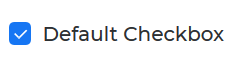
\includegraphics[scale=0.5]{M4_Vaadin_ChkBox}
	\caption{Checkbox generado por Vaadin}\label{fig:M5_Vaadin_ChkBox}
\end{figure}
\FloatBarrier

\subsection{Ventajas e inconvenientes}
Entre las ventajas en el uso de esta herramienta se encuentran:
\begin{itemize}
	\item Supone no cambiar de lenguaje de programación
	\item Permite crear interfaces utilizando Java, HTML o una combinación de ambos. También permite estilizar la aplicación con CSS
	\item Presenta una amplia librería de componentes \footnote{\url{https://vaadin.com/components}} de interfaz gráfica gratuitos que se adaptan a la gran mayoría de necesidades
	\item Permite personalizar los componentes e incluso publicarlos en el directorio Vaadin \footnote{\url{https://vaadin.com/directory/search}} para compartirlos con el resto de la comunidad.
	\item Es fácil de aprender a utilizar esta herramienta y tiene documentación de gran calidad y un buen soporte técnico
	\item Se integra con Maven y Eclipse
\end{itemize}

Y entre los inconvenientes:
\begin{itemize}
	\item Para usar componentes avanzados, se debe adquirir una licencia. Uno de estos componentes que hubiera ayudado en el desarrollo del programa es \textit{Vaadin Designer}, que se puede instalar como plugin en Eclipse y permite desarrollar la interfaz gráfica de una forma más visual
	\item Se puede complicar el mantener un modelo que separe la interfaz de la parte lógica al tener ambas partes escritas en un mismo lenguaje
\end{itemize}

\subsection{Configuración adicional para poder utilizar la aplicación en Internet Explorer}

Para poder ejecutar la aplicación en Internet Explorer 11 ha sido necesario añadir un perfil de producción en el fichero \ruta{pom.xml}:\\
\begin{minipage}{\linewidth}
{\tiny \begin{lstlisting}
<profiles>
  <profile>
    <id>production</id>
    <properties>
      <vaadin.productionMode>true</vaadin.productionMode>
    </properties>
    <dependencies>
      <dependency>
        <groupId>com.vaadin</groupId>
        <artifactId>flow-server-production-mode</artifactId>
      </dependency>
    </dependencies>
    <build>
      <plugins>
        <plugin>
          <groupId>com.vaadin</groupId>
          <artifactId>vaadin-maven-plugin</artifactId>
          <version>${vaadin.version}</version>
          <executions>
            <execution>
              <goals>
                <goal>copy-production-files</goal>
                <goal>package-for-production</goal>
              </goals>
            </execution>
          </executions>
        </plugin>
      </plugins>
    </build>
  </profile>
</profiles>
\end{lstlisting}}
\end{minipage}
y es necesario compilar con la opción \textit{-Pproduction-mode}.

\subsection{Elementos de terceros}

Para la interfaz se ha utilizado un componente del \textit{Vaadin Directory} creado por terceros. Se trata de un diálogo de confirmación y se puede encontrar en el siguiente enlace: \url{https://vaadin.com/directory/component/confirm-dialog}. Este diálogo se ha personalizado para determinadas funcionalidades de la aplicación y facilitar el uso del mismo. Por ejemplo se ha definido una clase de envoltura: \textit{ConfirmDialogWrapper} y también de han definido algunos diálogos a partir de la clase de envoltura como se muestra en la Fig. \ref{fig:M5_Vaadin_DialogoConfirm}

\begin{figure}[!h]
	\centering
	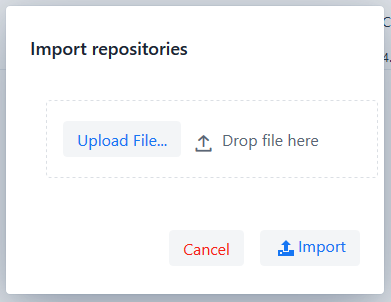
\includegraphics[width=0.45\textwidth]{M5_Vaadin_DialogoConfirm}
	\caption{Dialogo de confirmación personalizado a las necesidades de la funcionalidad}\label{fig:M5_Vaadin_DialogoConfirm}
\end{figure}
